\chapter{Algoritmo de detecci\'on de picos dobles}
\label{ap:doublePeakDet}

A continuaci\'on se describe el algoritmo utilizado para detectar estaciones con estructuras de doble pico en el an\'alisis de ES:

\begin{enumerate}
	 \item \textbf{Encontrar picos sobre \cant{0.6}{VEM_{peak}}:} para cada PMT activo se divide la traza en ventanas de 8 bines. Dentro de cada ventana se busca el bin cuya señal máxima y se define como un pico si su señal se encuentra por encima de los \cant{0.6}{VEM_{peak}}.
	 \item \textbf{Encontrar bloques de señal:} si en el paso 1 se etiqueta más de más de un bin como pico se busca en sus bines intermedios.
	 Se cuenta el número de bines que tienen señales por debajo del $30\%$ del mínimo pico encontrado. 
	 Si existen entre picos más de 6 bines consecutivos o más que cumplan la condición anterior, se divide la señal en el primer bin de ese grupo.
	 La figura \ref{fig:doublePeakEvent2} esquematiza esta etapa del algoritmo para el PMT número 1 de la estación 882 del evento 2629688.
	 %
	 \begin{figure}[ht]
	 \begin{center}
	 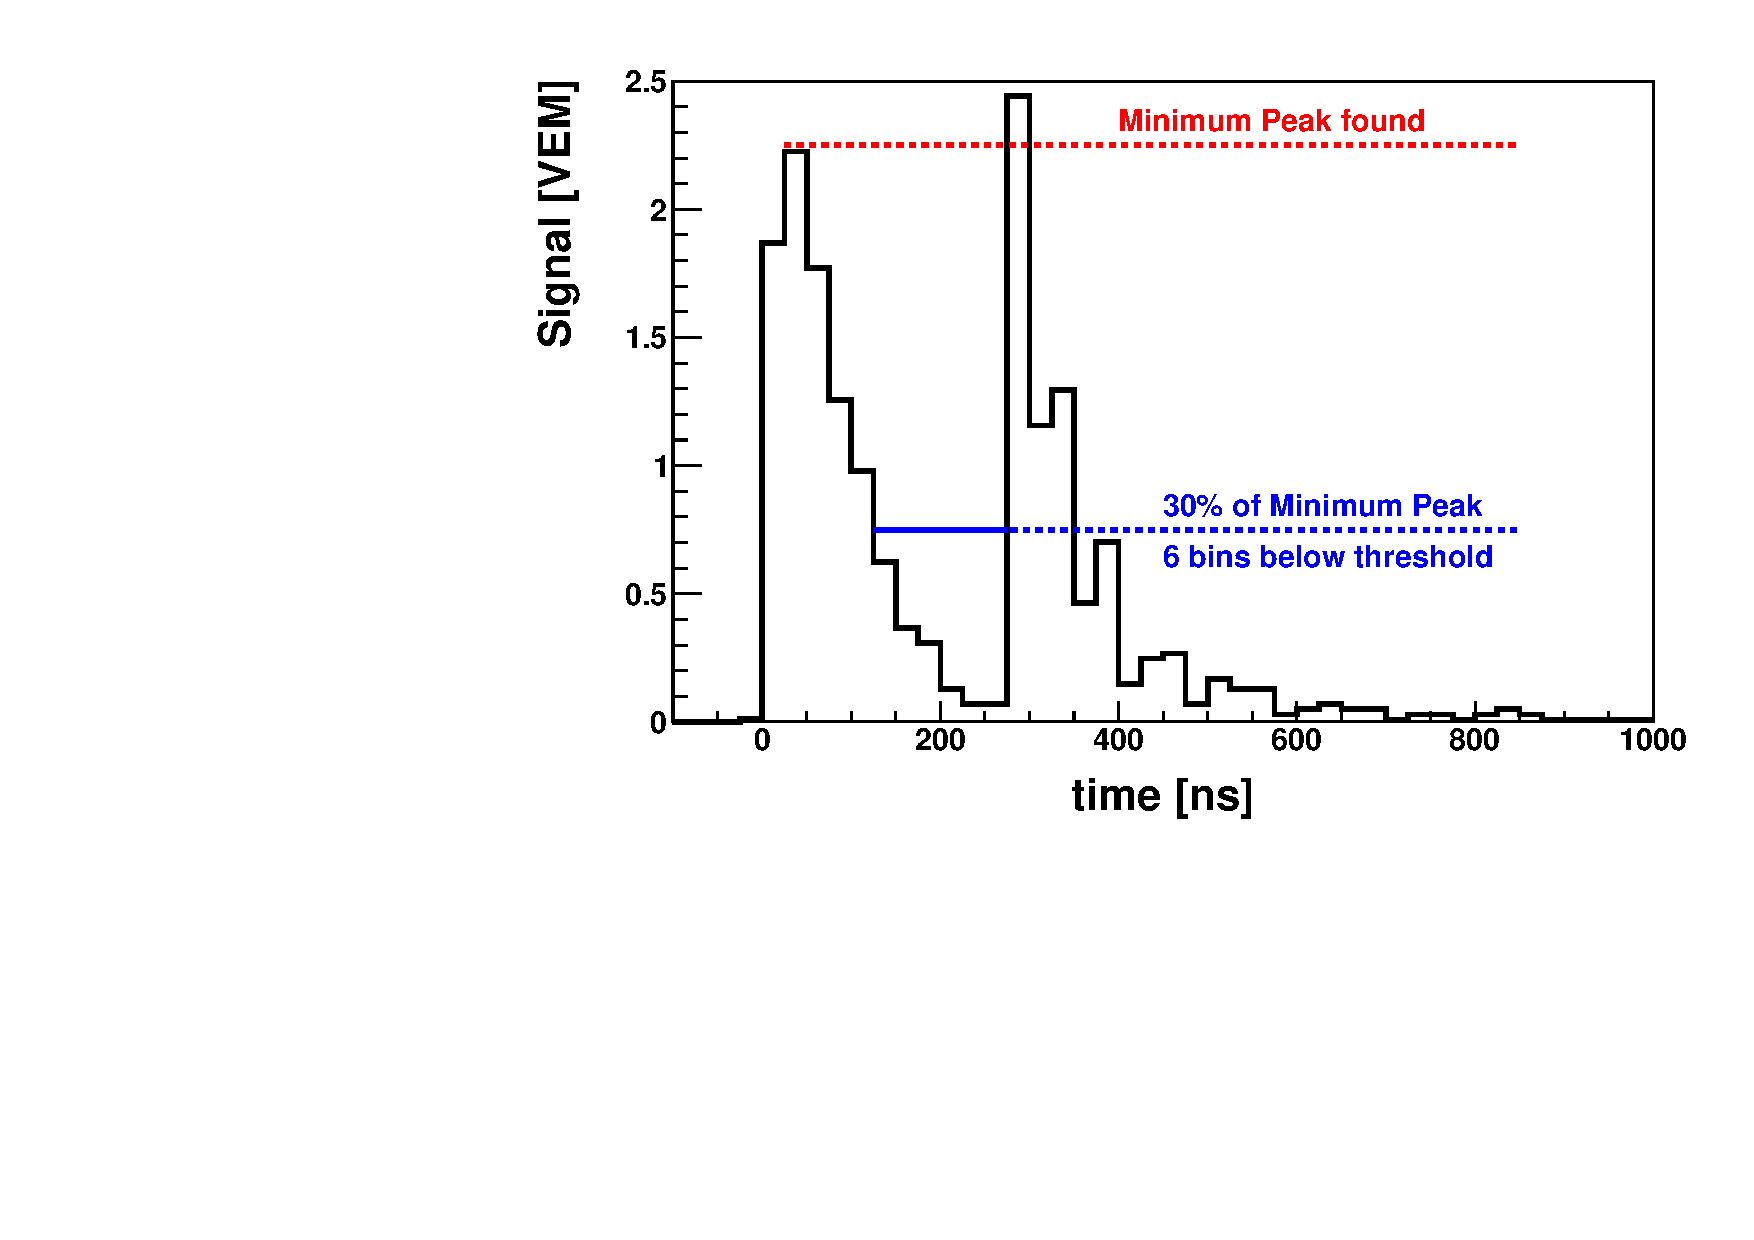
\includegraphics[width=0.7\textwidth]{fig/seleccionAuger/ev2629688_pmt1_anode}
	\caption{PMT 1 de la estación 882 del evento 2629688. La traza presenta dos picos con 6 bines contiguos por debajod el umbral establecido.}
	\label{fig:doublePeakEvent2}
	\end{center}
	\end{figure}
	 %
	 \item \textbf{Cálculo del AoP de los bloques:} si existe más de un bloque, se calcula la variable AoP integrando la señal hasta 8 bines despues del pico o hasta que la señal caiga por debajo de los \cant{0.2}{VEM_{peak}}.
	 \item \textbf{Etiquetar trazas dominadas por picos:} si la suma de la señal integrada de los bloques se encuentra por debajo del $90\%$ de la señal interada total del PMT, no se lo etiqueta.
	 \item \textbf{Contar bloques con AoP$<1.5$:} Sin importar el numero de partículas que atraviecen el tanque, si el desfasaje es pequeño (típico de los frentes muónicos en eventos pequeños) se cumple que ${\rm AoP}\sim 1$. Si se encuentran varios picos que cumplan AoP$<1.5$ se etiqueta el PMT.
	 \item \textbf{Etiquetar la estación:} si una estación cuenta con más de un PMT etiquetado se rechaza y no se utiliza para calcular \aop{}.
\end{enumerate}
